We now develop methodology to estimate $\bopt$ and $\cbs$ over the
dimensions of total training tokens $D$, total compute FLOPs $C$, and
validation loss $L$. Results show power-law scaling of both $\bopt$
and $\cbs$ with $D$, enabling estimation of $\cbs$ at scale via a
small number of test runs at modest budgets.

\subsection{Background: $\bopt$ and $\bcrit$}\label{sec:cbs_background}

\paragraph{$\bopt$}

As noted above, recent work has pursued an \emph{optimal} $B$: the $B$
achieving lowest loss given $N, D$.
%
\citet{hu2024minicpm} fit $\bopt$ using a power law in
(estimated) loss, and use $\mup$ to set $\eta$.
%
%$B$ and $\eta$ can be tuned together at small scales and transferred
%to larger runs~\citep{sengupta2023jais},
%
Joint power laws for optimal $\eta$ and $B$ have also been
fit~\citep{bi2024deepseek,porian2024resolving,carbonneaux2025cwm}.
E.g.,
\citet{bi2024deepseek} estimated \mbox{$\bopt = 0.292 C^{0.3271}$} (in tokens);
we refer to this fit as $\bdeepseek$ below.
%
\citet{li2025predictable} found $\etaopt$ to scale in $N, D$, while $\bopt$ primarily scales in $D$.
%
Qwen2.5~\citep{yang2024qwen2_5} also report studying how $\etaopt$ and
$\bopt$ scale with $N$ and $D$ (across dense and mixture-of-expert
LLMs), but without further details.

%jais: ''we tuned the optimal values for batch size and learning rate
%on a 40M-parameter model, and transferred the best values to our
%13B-parameter model.''

\paragraph{$\bcrit$}

Let $D$ be the number of training tokens required to reach target loss
$\lhat$ when using a batch size of $B$.  \mbox{$S = {D}/{B}$} is the
corresponding number of optimization steps.
%
Doubling a small $B$ doubles per-step gradient information; $\lhat$
can be reached in half the optimization steps, using the same total
$D$ (so-called ``perfect
scaling''~\citep{ma2018power,shallue2019measuring}).
%
But as $B$ increases further, step-wise gradient information becomes
more and more redundant: eventually, much larger $D$ is required to
reach $\lhat$, and $S$ decreases only marginally.
\citet{mccandlish2018empirical} show that $\langle D, S \rangle$ pairs
can be well fit by the equation:
%
\begin{equation}\label{eq:tradeoff}
S/\smin - 1 = (D/\dmin - 1)^{-1}
\end{equation}
where $\smin$ and $\dmin$ are parameters to be fit.  Intuitively,
$\dmin < D$ is the asymptotically minimum number of tokens that can
reach $\lhat$ (achieved with $\bopt$) and $\smin < S$ is the
asymptotically minimum number of \emph{steps} that can reach $\lhat$
(achieved as $B \rightarrow \infty$).
%These are also the asymptotes in \cref{fig:d_s_cartoon}.
\cref{eq:tradeoff} defines a hyperbolic curve, like those in
\cref{fig:cbs_panels}, where $B$ controls the position on the curve
and can be set depending on the importance of time (higher $B$
$\rightarrow$ higher $D$, lower $S$) or compute (lower $B$
$\rightarrow$ lower $D$, higher $S$).

\begin{definition}
\label[definition]{def:cbs}
The \emph{critical batch size} at $\lhat$ is defined from the fit
of \cref{eq:tradeoff} as $\cbs$=${\dmin}/{\smin}$.
\end{definition}

%; it is the largest \emph{useful} $B$ for
%training: the largest $B$ before $D$ rapidly increases.

From \cref{eq:tradeoff}, we can derive (\cref{sec:cbs_derivations}),
for a given $B$, the $D$ needed compared to $\dmin$:
\begin{equation}\label{eq:s_extra}
D = \dmin(1 + B/\cbs)
\end{equation}
%
\cref{eq:s_extra} implies that when $B$=$\cbs$, we require
$2\times\dmin$ tokens (and $2\times\smin$ steps) to reach $\lhat$.  $\cbs$ is a
\emph{transition} point along the $D$ vs.\ $S$ curve: for $B
> \cbs$, much higher $D$ is needed for only small reductions in $S$
(\cref{fig:cbs_panels}).
%
% McCandlish also refer to $\cbs$ as the largest \emph{useful} batch size.
%
%In this way, $\cbs$ is not ``optimal'' in the sense of achieving the
%lowest loss for a given $N$ and $D$.  Rather,
\citet{kaplan2020scaling} refer to $\bcrit$ as the \emph{optimal compromise}
between time and compute.  They determine $\cbs$ at smaller scales and
fit a power law for $\cbs$ as a function of $\lhat$.

\cref{eq:s_extra,eq:tradeoff} also imply $\bopt$ is theoretically equal to 1.
%, i.e., the batches should be more and more compute-efficient.
In practice, loss degrades below a particular
$\bopt$~\citep{hu2024minicpm,bi2024deepseek,porian2024resolving}, a
finding that ``appears to contradict the conventional wisdom'' about
$\bcrit$~\citep{porian2024resolving}.
%our results appear to contradict the conventional wisdom about the
%existence of a critical batch size [49, 61, 36] below which every batch size is good, finding instead% an
%optimal batch size below which performance degrades.
%
With well-tuned $\lambda$, we find small differences in loss across
small $B$, suggesting \cref{eq:tradeoff} may nevertheless provide a
good fit to observed data. \cref{sec:limitations} has further
discussion.

In recent work,
\citet{zhang2024how} define $\bcrit$ as the point where \mbox{$D = 1.2 \times \dmin$}.
They use a different training setup,
with a constant LR, weight averaging, and no weight decay.  Notably,
they observe little change in $\bcrit$ as $N$ varies at fixed $D$,
but, for a 302M model, find power-law scaling in $D$ as
\mbox{$\bcrit = 22.91 D^{0.47}$} (in tokens),
consistent with observed scaling across models at fixed TPP\@.
See \cref{sec:appendix_zhang} for further differences
with~\citet{zhang2024how}.

\subsection{Methods: estimating $\bopt$ and $\cbs$, and their scaling}\label{sec:cbs_methods}

\begin{figure}
  \noindent
\begin{minipage}[b]{0.32\textwidth}
  \centering
  %\begin{figure}
%  \centering
  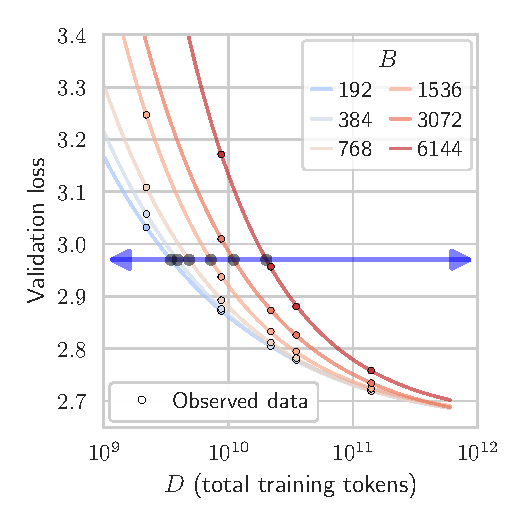
\includegraphics[trim={0.3cm 0.4cm 0.3cm 0.3cm}, clip, width=\linewidth]{pdffigs/241005.fitted_scale_law.gbs=multi.111M.l=2.97.pdf}
  %Scaling laws in $D$ for computing $\cbs$} (111M
  %scale): after training with different batch sizes, $B$, and
  %dataset sizes, $D$ (indicated by points on curves), we fit
  \caption{(111M): \textbf{Fitted $B$-specific power laws},
  $L_B(D)$, for inferring steps to reach target loss $\lhat$ (arrowed
  blue line).\label{fig:cbs_fitting}}
%
%    .  We can then
%    compute the amount of data needed to reach any target loss
  %    (arrowed line) for each batch size via $L_B^{-1}(D)$;
%  this
%    provides the points over which we fit \cref{eq:tradeoff} and
%    determine $\cbs$. .}}
%\end{figure}

    

\end{minipage}%
\hfill
\begin{minipage}[b]{0.64\textwidth}
  \centering
  %\begin{figure}
%  \centering
  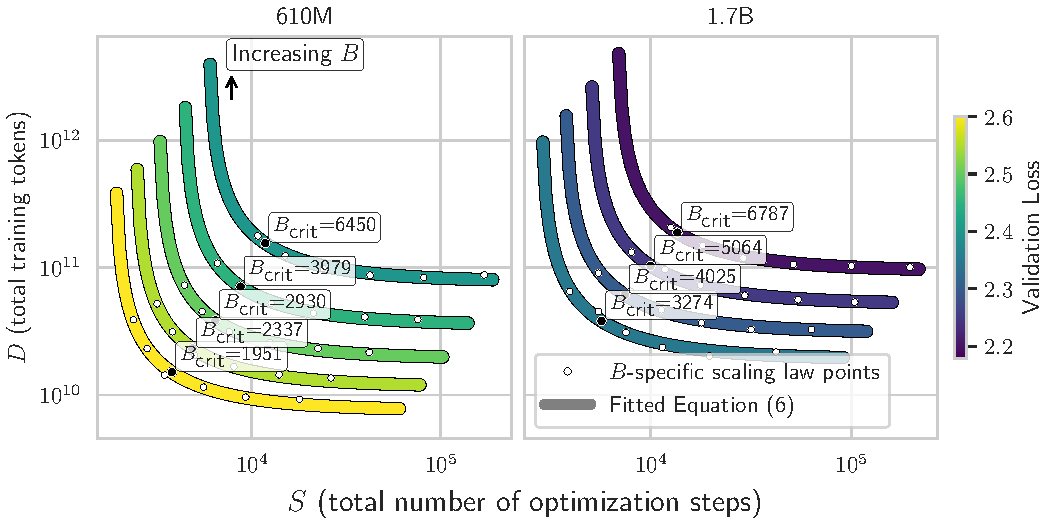
\includegraphics[trim={0.1cm 0.1cm 0.1cm 0.1cm}, clip, width=\textwidth]{pdffigs/loss_data.241005_batchsizes.twopanel_cbs.pdf}
  \caption{\textbf{\cref{eq:tradeoff} fits observed data well}:
    Increasing $B$ (moving leftward along curves) decreases
    optimization steps (x-axis), but requires more tokens (y-axis) to
    reach target loss (in color).  $\cbs$ is the transition point along
    each fitted curve.
    % Across model scales, we see that $\cbs$ does not correlate with
    % loss, but rather the number of tokens processed, $D$ (shared
    % y-axis).
    \label{fig:cbs_panels}}
%\end{figure}

\end{minipage}
\end{figure}

\paragraph{Estimating $\bopt$}

We use the same experimental settings as \cref{sec:lambda_experimental}.
%
%As in \citet{shallue2019measuring}, ``We try to avoid making
%assumptions about how the optimal metaparameters vary as a function of
%batch size'' so even though we found good rules for this, we actually
%tuned HPs at each batch size at most of our model scales.  More
%details in appendix.
%
To ensure good HPs, we sweep $\lambda$ by factors of $2\times$ at each
$B$, $D$, $N$, except at the largest scales (see
Appendix \cref{tab:train_steps}) where we set $\lambda$ via the
projected value from \cref{eq:lambdaopt}.
%
In all figures, $B$ is reported in units of \emph{sequences}.

\paragraph{Estimating $\cbs$}\label{sec:estimating_bcrit}

%We first discuss how we fit $\cbs$ for a particular model with a
%particular loss target, $\lhat$.  We then describe how we fit a scaling
%law for $\cbs$.

Unlike $\bopt$, measuring $\cbs$ requires training models with
different $B$ \emph{to the same $\lhat$}.
%
Unfortunately, we do not know \emph{a priori} how many steps are
required to reach $\lhat$, yet we need this information to configure a
LR schedule that reaches its minimum value on the final step (the
typical setup, shown to be consequential in prior
work~\citep{hoffmann2022empirical,hagele2024scaling}).
%
Unfortunately, it is not feasible to \emph{search} for the precise
steps needed, i.e., by conducting training runs with different
schedules/step budgets.

\citet{mccandlish2018empirical} address this issue by performing
a single training run at a constant LR, while \citet{zhang2024how}
also use a constant LR, but use weight averaging to frequently
generate higher-quality checkpoints for evaluation
(\cref{sec:appendix_zhang}).

In contrast, we desired a method agnostic to the LR schedule.
%
We achieved this by fitting batch-size-specific power laws that model
how \emph{loss} scales with $D$.
%
These laws allow us to accurately \emph{interpolate} the $D$ required
to reach $\lhat$.  \cref{fig:cbs_fitting} depicts, for different $B$
and a given $\lhat$, the interpolated $D$ values (intersection points
of arrowed line and fitted loss curves).  The full process to obtain
$\cbs$ at $\lhat$ is:
\begin{enumerate}
\item For each $B$, train over different $D$, and
subsequently fit a $B$-specific power law \mbox{$L_{B}(D) = \irr + \dconst D^{-\beta}$}
on the resulting loss values (fitted curves in \cref{fig:cbs_fitting}).
\item Use fitted $L_{B}(D)$ to infer the $\dinfer$ needed to reach $\lhat$ as:
\mbox{$\dinfer = L_{B}^{-1}(\hat{L}) = (\nicefrac{\dconst}{\hat{L}-\irr})^{\frac{1}{\beta}}$}.
\item Fit \cref{eq:tradeoff} on the resulting $\langle \dinfer, S$=${D}/{B} \rangle$ pairs, and obtain $\cbs = {\dmin}/{\smin}$.
\end{enumerate}
%
This method makes no assumptions about the LR schedule or optimizer,
while enabling measurement of $\cbs$ at arbitrary losses without
re-training.
%
\cref{sec:appendix_estimating_cbs} provides further details,
%
including fits of $L_{B}(D)$ at other model scales
(\cref{fig:quad_cbs_fitting}) and a summary of the full procedure
(\cref{alg:cbs_fitting}).

\paragraph{$\bopt$ and $\cbs$ scaling}

We collect $\bopt$ across different $N$ and $D$, and fit a power law
in both data $D$ and compute $C$ (via the standard approximation
$C \approx 6ND$~\citep{kaplan2020scaling,hoffmann2022empirical}).
%
For $\bcrit$, we use the procedure described above to estimate $\cbs$
across multiple $\lhat$, across different $N$.  From each $\cbs$
estimate, we obtain a pair $\langle \dmin, \cbs \rangle$.
%
We propose that $\cbs$ follows a power law in $\dmin$, according to:
\begin{equation}\label{eq:cbs_scaling}
  \cbs(\dmin) = {\ccbs} \cdot \dmin^{\mcbs}
\end{equation}
Where $\ccbs$ and $\mcbs$ are fit on the $\langle \dmin, \cbs \rangle$
pairs.
%In the following results, we find strong fits
%to \cref{eq:cbs_scaling} over experimental data.

\subsection{Results: $\bopt$ and $\bcrit$}\label{sec:results_cbs}

\begin{figure}[H]
    \centering
    \begin{minipage}{0.33\textwidth}
        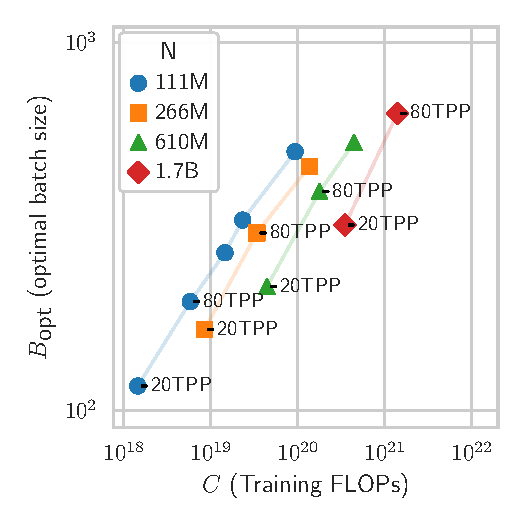
\includegraphics[trim={0.3cm 0.4cm 0.3cm 0.3cm}, clip, width=\linewidth]{pdffigs/bopt_scaling_law.mydata.C.pdf}
    \end{minipage}\hfill
    \begin{minipage}{0.33\textwidth}
        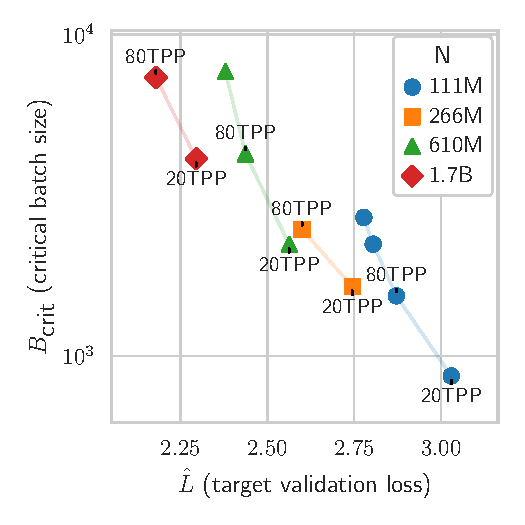
\includegraphics[trim={0.3cm 0.4cm 0.3cm 0.3cm}, clip, width=\linewidth]{pdffigs/loss_data.241005.cbs_scaling.target_loss.pdf}
    \end{minipage}\hfill
    \begin{minipage}{0.33\textwidth}
        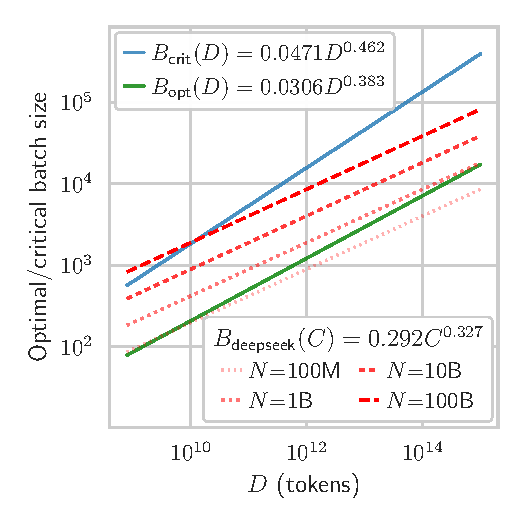
\includegraphics[trim={0.3cm 0.4cm 0.3cm 0.3cm}, clip, width=\linewidth]{pdffigs/b_all_scaling.pdf}
    \end{minipage}
    \caption{Prior work suggests $\bopt$ scales in $C$ ($\leftfig$)
      and $\bcrit$ in loss ($\middlefig$), but \emph{this only holds
      at a fixed $N$/TPP} (same data as \cref{fig:hook}
      $\middlefig$/$\rightfig$); \cref{fig:hook} shows scaling in $D$
      is the fundamental relationship.
      %
      Plotting $\bdeepseek(C)$ law from~\citet{bi2024deepseek}
      ($\rightfig$), but over $D$ (using $C \approx 6ND$ to obtain $C$
      for the spurious dependence on $N$), we see
      \citet{bi2024deepseek} used generally efficient $B$ values
      (i.e., within the $\bopt < B < \bcrit$ regime) despite fitting $C$
      rather than $D$ ($\bopt$ and $\bcrit$ lines from
      \cref{fig:hook}).\label{fig:related}}
\end{figure}


\finding{\cref{eq:tradeoff} provides a decent fit to the trade-off
  between training time and compute.}

Across different model scales and loss targets, we consistently find
that our $\langle D, S \rangle$ pairs fit \cref{eq:tradeoff} well
(examples in \cref{fig:cbs_panels}, appendix
\cref{fig:quad_cbs_fits}).
%
Fits are worse at very small $B$, as noted above: smaller batches are
not monotonically more efficient; \cref{sec:limitations} discusses
some potential reasons for this.

% Notably, the horizontal alignment of similar $\cbs$ in
%\cref{fig:cbs_panels} already suggests $\cbs$ does not depend on the
%loss (in color), but rather on number of tokens processed (shared
%y-axis).

%\input{figures/fig_cbs_scaling_zhang.tex}

\finding{$\bopt$ and $\cbs$ obey power laws in $D$ and $\dmin$, not in $C$ or $L$.}

$\bopt$ and $\cbs$ datapoints fit power laws quite well
(\cref{fig:hook}, $\middlefig$, $\Rtwo$=0.984) and (\cref{fig:hook},
$\rightfig$, $\Rtwo$=0.940).
%
10\textsuperscript{th} and 90\textsuperscript{th} percentiles over all
points are (0.367, 0.391) for fitted $\mbopt$ and (0.491, 0.526) for
$\mcbs$ (computed as in \cref{sec:tema_results}).  Note $\mcbs$ is
higher when fitted over \emph{all} points (as opposed to only
small-scale runs), partly reflecting the 111M points trending lower as
TPP increases.

Our fitted $\bcrit$ power law exponent is very close to that
from~\citet{zhang2024how}: 0.47 vs.\ 0.462.  Given the many
differences in approach (including dataset, use of weight decay, LR
schedule, etc., \cref{sec:appendix_zhang}), this agreement suggests
the fundamental relationship of $\bcrit$ with $D$ persists across such
differences.
%Moreover, given the significant implications of $\bcrit$'s
%fundamental scaling behavior, it is valuable, scientifically and
%practically, that different approaches independently measure a
%similar scaling relationship.

\cref{fig:related} ($\leftfig$) plots $\bopt$ versus $C$ and
\cref{fig:related} ($\middlefig$) gives $\bcrit$ versus $L$ using
the same data as in \cref{fig:hook}.
%
In each case, a power law does not fit all points (as proposed
previously), but points at the same $N$, or same TPP, can roughly be
linked by (parallel) lines.  This is a consequence of power-law
scaling in $D$ (see \cref{sec:appendix_loss_scaling}).
%
That is, scaling in $D$ is the fundamental scaling relationship:
$\bopt$ and $\bcrit$ both scale in $D$ regardless of TPP, model size,
or loss---it is only when using another (misleading) scaling factor
such as $C$ or $\lhat$ that TPP or model size appears important, as in
these plots.

\cref{fig:related} ($\rightfig$) compares the recommended batch sizes
from $\bdeepseek$ to those from $\bopt$ and $\bcrit$.  Since
$\bdeepseek$ scales in $C$, it is larger for larger $N$.  Over a range
of modern model sizes, $\bdeepseek$ values generally fall between our
projected $\bopt$ and $\bcrit$, varying in the extent to which they
are compute-efficient (close to $\bopt$) or time-efficient (close to
$\bcrit$).
%In the next section, we develop a targeted approach to find $N$, $D$,
%and $B$ settings achieving an optimal balance of time and compute.

\finding{Weight decay affects the accuracy of fitted batch size scaling laws.}\label{finding:wd_bopt}

Prior work has typically held $\lambda$ fixed when fitting batch-size
scaling laws \citep{bi2024deepseek,porian2024resolving,zhang2024how}.
Doing so not only degrades loss (\cref{sec:lambda}) but also reduces
the accuracy and generality of the fitted scaling relationships.  We
demonstrate this in appendix \cref{tab:wd_bopt}: rather than tuning
$\lambda$ for each $B$, we train with several fixed $\lambda$ values
across all runs.
%
As \cref{tab:wd_bopt} shows, increasing $\lambda$ systematically
raises the estimated $\bopt$.  This arises because the fundamental
scaling variable is the AdamW timescale $\tema = B /
(\eta \lambda D)$: when $\lambda$ increases, the batch size that
minimizes loss must increase proportionally to preserve the optimal
$\tema$.
%
In Appendix~\ref{sec:app_wd_affects_b}, we show that these effects
distort the fitted power-law slope and reduce fit quality ($R^{2}$),
leading to scaling laws that do not generalize to large-scale
training---even if the same fixed weight decay is used there.  When
$\lambda$ is tuned to maintain the optimal timescale (final row
of \cref{tab:wd_bopt}), the resulting $\bopt$ follows a clean and
accurate power law.

Similar distortions occur for $\bcrit$ when $\lambda$ is fixed 
(Appendix~\ref{sec:app_wd_affects_b}).

\takeaway{You can estimate $\bopt$ and $\cbs$ for a small $N$ by training with
  different $B$, $D$ and $\lambdaopt$, and computing loss.  From
  there, $\bopt \propto D^{0.4}$ and $\cbs \propto D^{0.5}$.  At
  larger $N$ and $D$, \cref{eq:s_extra} lets you estimate trade-offs in
  FLOPs ($\propto D$) vs.\ training time ($\propto S = {D}/{B}$) at
  different $B$.}
